\documentclass[a4paper,12pt]{article}

\title{ Opracowanie pisemne zestawu egzaminacyjnego nr 4 }
\author{ Analiza Numeryczna | Aleksander Tudruj }
\date{ 27 stycznia 2024 }

%\pagestyle {empty} %wyłącza numerowanie stron
\usepackage[super]{nth}

\usepackage[T1]{fontenc}
\usepackage[utf8]{inputenc}

\usepackage[usenames,dvipsnames]{xcolor}
\definecolor{Nblue}{RGB}{0, 72, 110}
\definecolor{Lblue}{RGB}{236, 250, 255}

\usepackage[headheight=0cm, left=1cm, right=1cm, top=2cm, bottom=2cm]{geometry}
\usepackage{amsfonts,amsmath}
\usepackage{amsmath,amsthm,amssymb}
\usepackage{gensymb}
\usepackage{enumitem}
\usepackage{stmaryrd}
\usepackage{blindtext}
\usepackage{hyperref}

\newcommand{\stirSet}[2]{\left\{\begin{array}{c}
                                    \!\!#1\\ \!\!#2
\end{array}\!\!\right\}}
\newcommand{\stirPerm}[2]{\left[\begin{array}{c}
                                    \!\!#1\\ \!\!#2
\end{array}\!\!\right]}
\newcommand{\stirBin}[2]{\left\left(\begin{array}{c}
                                        \!\!#1\\ \!\!#2
\end{array}\!\!\right\right)}
\newcommand{\set}[1]{\left\{ #1\right\}}
\newcommand{\floor}[1]{\lfloor #1\rfloor}
\newcommand{\ceil}[1]{\lceil #1\rceil}
\newcommand{\suma}[2]{\sum \limits_{#1}^{#2} }
\newcommand{\infsum}[1]{\sum_{#1}^{\infty}}
\newcommand{\mysuma}[2]{\sum_{#1}^{#2}}
\newcommand{\myroot}[2]{\sqrt[\leftroot{0}\uproot{0}#1]{#2}}

\newcommand{\vect}[1]{\overrightarrow{#1}}
\newcommand{\af}[1]{\text{af}{#1}}
\newcommand{\lin}[1]{\text{lin}{#1}}
\newcommand{\R}[0]{\mathbb{R}}
\newcommand{\C}[0]{\mathbb{C}}
\newcommand{\N}[0]{\mathbb{N}}
\newcommand{\Z}[0]{\mathbb{Z}}
\newcommand{\Q}[0]{\mathbb{Q}}
\newcommand{\mat}[1]{\left[\begin{matrix}
                               #1
\end{matrix}\right]}
\newcommand{\operacje}[1]{\begin{matrix}
                              #1
\end{matrix}}
\newcommand{\row}[0]{\text{R}}
\newcommand{\uklad}[1]{\begin{cases}
                           #1
\end{cases}}
\newcommand{\la}[0]{\left\left(}
\newcommand{\ra}[0]{\right\right)}

\newcommand{\myeq}[1]{\mathrel{\stackrel{\makebox[0pt]{\mbox{\normalfont\tiny #1}}}{=}}}

\usepackage { graphicx }

\usepackage{listings}
\usepackage{color}

\usepackage{multicol}

\definecolor{dkgreen}{rgb}{0,0.6,0}
\definecolor{gray}{rgb}{0.5,0.5,0.5}
\definecolor{mauve}{rgb}{0.58,0,0.82}

\lstset{frame=tb,
    language=C++,
    aboveskip=3mm,
    belowskip=3mm,
    showstringspaces=false,
    columns=flexible,
    basicstyle={\small\ttfamily},
    numbers=none,
    numberstyle=\tiny\color{gray},
    keywordstyle=\color{blue},
    commentstyle=\color{dkgreen},
    stringstyle=\color{mauve},
    breaklines=true,
    breakatwhitespace=true,
    tabsize=2
}

\usepackage{caption}
\usepackage{subcaption}


\newcommand{\lmax}[1]{\lambda_{\text{max}}(#1)}
\newcommand{\lmin}[1]{\lambda_{\text{min}}(#1)}
\newcommand{\condtwo}[1]{\text{cond}_2(#1)}

\usepackage{multicol}

\usepackage{listings}
\usepackage{color}

\definecolor{dkgreen}{rgb}{0,0.6,0}
\definecolor{gray}{rgb}{0.5,0.5,0.5}
\definecolor{mauve}{rgb}{0.58,0,0.82}

\lstset{frame=tb,
  language=Python,
  aboveskip=3mm,
  belowskip=3mm,
  showstringspaces=false,
  columns=flexible,
  basicstyle={\small\ttfamily},
  numbers=none,
  numberstyle=\tiny\color{gray},
  keywordstyle=\color{blue},
  commentstyle=\color{dkgreen},
  stringstyle=\color{mauve},
  breaklines=true,
  breakatwhitespace=true,
  tabsize=2
}

\makeatletter
\renewcommand*\env@matrix[1][*\c@MaxMatrixCols c]{%
  \hskip -\arraycolsep
  \let\@ifnextchar\new@ifnextchar
  \array{#1}}
\makeatother

\newenvironment{Figure}
  {\par\medskip\noindent\minipage{\linewidth}}
  {\endminipage\par\medskip}

\begin{document}
\maketitle

\section*{Zagadnienie 1}
Wpływ rozkładu wartości własnych macierzy $A$ na zbieżność różnych metod iteracyjnych rozwiązywania układu $Ax = b$.

\subsection*{Rozumowanie}

Rozważymy metody iteracyjne oparte o metodę Kryłowa. Zbieżność
tych metod ściśle zależy od wartości własnych macierzy $A$, gdy rozwiązujemy
układ $Ax = b$.

\subsubsection*{Metoda CG}

Rozważmy macierz $A$, która jest symetryczna i dodatnio określona.
Posiada ona rozkład $A = V \Lambda V^T$, gdzie $\Lambda = \text{diag}(\lambda_i)$,
a $V$ składa się z wektorów własnych.
Wówczas definiujemy $\kappa = \condtwo{A} = \frac{\lmax{A}}{\lmin{A}}$
i mówimy, że po $k$ iteracjach metody CG otrzymamy
$$
    ||x_k - x^*||_A \leq 2 \left( \frac{\sqrt{\kappa} - 1}{\sqrt{\kappa} + 1} \right)^k ||x_0 - x^*||_A.
$$

Gdy $\kappa$ jest duże, to metoda CG będzie wolno zbieżna, lecz gdy wartości własne
będą \textit{blisko} siebie, to metoda będzie szybko zbieżna. Co więcej,
jeżeli $A$ ma dokładnie $m$ różnych wartości własnych, to metoda CG zbiega
do rozwiązania w co najwyżej $m$ iteracjach w arytmetyce dokładnej.

\subsubsection*{Metoda Najszybszego Spadku}

Podoba rzecz tyczy się metody najszybszego spadku. Wówczas kolejne błędy będą spełniać
następującą zależność
$$
    ||x_k - x^*||_A \leq \frac{\kappa - 1}{\kappa + 1} ||x_0 - x^*||_A.
$$

Zbieżność tej metody jest znacznie wolniejsza niż metody CG i również zależy od
wartości własnych macierzy $A$.

\subsubsection*{Metoda Richardsona}

Metoda Richardsona z parametrem $\tau \in \R$ jest metodą iteracyjną opisaną wzorem
$$
    x_{k+1} = x_k + \tau (b - Ax_k).
$$

Popatrzmy na błąd występujący w metodzie Richardsona. Wiemy, że $x^*$ będące dokładnym
rozwiązaniem układu równań spełnia $Ax^* = b$. Rozpiszmy więc z definicji
\begin{align*}
    x_{k+1} - x^* & = x_k + \tau (b - Ax_k) - x^* \\
                  & = x_k - x^* + \tau (b - Ax_k)  \\
                  & = x_k - x^* + \tau (Ax^* - Ax_k) \\
                  & = x_k - x^* - \tau (Ax_k - Ax^*) \\
                  & = (I - \tau A)(x_k - x^*).
\end{align*}
Możemy więc zapisać
$$
    ||x_{k+1} - x^*|| = ||I - \tau A|| \cdot ||x_k - x^*||.
$$
Wiemy jednak, że $A = V \Lambda V^T$, więc
$$
    ||I - \tau A|| = ||VV^T - \tau V\Lambda V^T|| = ||V(I - \tau \Lambda)V^T|| = ||I - \tau \Lambda||.
$$

Z własności metod stacjonarnych wiemy, że metoda jest zbieżna, jeżeli
$$
    ||I - \tau \Lambda|| < 1.
$$

Jeżeli $$\tau = \frac{2}{\lmax{A} + \lmin{A}},$$ to metoda jest optymalna,
ale nie zawsze jesteśmy w stanie wyznaczyć wartości własne macierzy $A$.
Dlatego dobranie dobrego $\tau$ jest trudne.

\subsubsection*{Ściskanie macierzy}

W związku z tym, że metody wymienione wyżej są zależne od wartości
własnych macierzy $A$, to warto byłoby przekształcić macierz $A$ w macierz $B$,
która ma lepsze własności - w imię idei "Jak zadanie jest za trudne, to zmień zadanie".

Gdy szukamy odpowiedniej macierzy ściskającej musimy zwrócić uwagę na to,
aby macierz wynikowa nadal spełniała założenia naszej metody.
Na przykład w metodzie CG macierz musi być symetryczna i dodatnio określona.
Z kolei w metodzie GMRES jedynym ograniczeniem jest nieosobliwość macierzy.


\newpage
\section*{Zagadnienie 2}
Metoda dziel i rządź wyznaczania wartości własnych symetrycznej macierzy trójdiagonalnej. Jak w tej metodzie wyznaczać wektory własne.

\subsection*{Rozumowanie}

Wiemy, że $X A X^{-1}$ zachowuje wartości własne macierzy $A$. W szczególności będzie tak dla macierzy ortogonalnej $Q$, dla której $Q^T Q = I$.

Naszym celem jest wyznaczenie rozkładu $A = V\Lambda V^T$, takiego że $V^T V = I$, $\Lambda = \text{diag}(\lambda_i)$,
$V$ składa się z wektorów własnych, a $\lambda_1, \dots, \lambda_N$ to ciąg odpowiadających im wartości własnych.

Wykorzystamy metodę "dziel i rządź". Macierz $A$ jest symetryczna i trójdiagonalna, więc możemy zapisać ją w następujący sposób
$$
    A = \begin{bmatrix}[ccc|ccc]
        a_1 & b_1    &        &           &           &           \\
        b_1 & \ddots & \ddots &           &           &           \\
            & \ddots & a_m    & b_m       &           &           \\
        \hline
            &        & b_m    & a_{m + 1} & \ddots    &           \\
            &        &        & \ddots    & \ddots    & b_{N - 1} \\
            &        &        &           & b_{N - 1} & a_N
    \end{bmatrix}
    = $$$$ =
    \begin{bmatrix}[ccc|ccc]
        a_1 & b_1    &           &                 &           &           \\
        b_1 & \ddots & \ddots    &                 &           &           \\
            & \ddots & a_m - b_m &                 &           &           \\
        \hline
            &        &           & a_{m + 1} - b_m & \ddots    &           \\
            &        &           & \ddots          & \ddots    & b_{N - 1} \\
            &        &           &                 & b_{N - 1} & a_N
    \end{bmatrix}
    +
    \underbrace{
        \begin{bmatrix}[ccc|ccc]
             &   &     &     &   & \\
             & 0 &     &     & 0 & \\
             &   & b_m & b_m &   & \\
            \hline
             &   & b_m & b_m &   & \\
             & 0 &     &     & 0 & \\
             &   &     &     &   &
        \end{bmatrix}
    }_{b_m \cdot u \cdot u^T}
    = $$$$ =
    \begin{bmatrix}[c|c]
        A_1 & 0   \\
        \hline
        0   & A_2 \\
    \end{bmatrix}
    + b_m \cdot u \cdot u^T.
$$
Parametr $m$ dobieramy tak, żeby przeciąć tę macierz mniej więcej w połowie, $m \approx \frac{N}{2}$.
Wektor $u$ jest sumą dwóch wektorów: $e_m + e_{m+1}$, tak aby w wyniku dawał macierz z samymi zerami,
poza małym kwadratem $2\times 2$.

Algorytm uruchamiamy rekurencyjnie dla mniejszych macierzy. Osobno rozpatrujemy przypadek,
gdy $N = 1$. Wówczas dla macierzy $\left[ a \right] \in \R^{1 \times 1}$ jej jedyną wartością
własną jest $a$, a wektorem własnym o normie 1 jest $e_1 \in \R^{1}$.

Zakładamy teraz, że rekurencyjnie uzyskaliśmy rozkłady mniejszych macierzy $A_1$ oraz $A_2$.
$$
    A_1 = V_1 \cdot \Lambda_1 \cdot V_1^T
    \quad
    A_2 = V_2 \cdot \Lambda_2 \cdot V_2^T.
$$
Wówczas macierz $A$ możemy zapisać jako
$$
    A = \underbrace{
        \begin{bmatrix}
            V_1 &     \\
                & V_2 \\
        \end{bmatrix}
    }_{\hat{V}}
    \underbrace{
        \left(
        \begin{bmatrix}
            \Lambda_1 &           \\
                      & \Lambda_2 \\
        \end{bmatrix}
        + b_m \cdot z z^T
        \right)
    }_{D}
    \underbrace{
        \begin{bmatrix}
            V_1 &     \\
                & V_2 \\
        \end{bmatrix}^T
    }_{\hat{V}^T},
    \text{ gdzie } z := \begin{bmatrix}
        V_1 &     \\
            & V_2 \\
    \end{bmatrix}^T \cdot u
$$

Zauważmy, że skoro $V_1$ i $V_2$ były ortogonalne, to diag$(V_1, V_2)$ też jest ortogonalne.
Jeżeli wyznaczymy rozkład własny macierzy $D = V_D \Lambda_D V_D^T$, to rozkładem
macierzy $A$ będzie $A = (\hat{V} V_D) \Lambda_D (\hat{V} V_D)^T$.
W implementacji algorytmu, aby odzyskać wektory własne macierzy $A$ wystarczy
skonstruować macierz $\hat{V}$ i domnożyć z prawej strony przez otrzymane $V_D$.

Teraz rozwiążemy problem znajdowania rozkładu dla macierzy $D + b_m \cdot zz^T$.

Jeżeli $b_m = 0$ lub $z = 0$, to wtedy wartości własne znajdują się na diagonali $D$,
a odpowiadające im wektory własne to kolejne wektory $e_i$, więc rozkładem będzie miał
postać $D = I D I$.

Załóżmy zatem, że $b_m \neq 0$ oraz $z \neq 0$.
Rozpatrzmy przypadki:

(1.) $z_i = 0$. Wówczas $(D + b_m zz^T)e_i = d_i e_i$, a zatem $(d_i, e_i)$ jest parą własną.

Możemy przepermutować wszystkie zera w wektorze $z$ na dół wektora za pomocą macierzy permutacji.
Weźmy taką macierz permutacji $P$, że $Pz=\begin{bmatrix} \hat{z} \\ 0 \end{bmatrix}$ i $\hat{z}$ nie posiada zer.

\begin{lstlisting}
# Wyznacz macierz permutacji przesuwania zer wektora z na dol
# Wektor z numerujemy od 1
def make_permutation_matrix(z, tol=eps):
    N := length(z)   # 1..N
    P := zeros(N, N)
    i := 1
    j := nnz(z) + 1
    for k = 1..N:
        if abs(z[k]) <= tol:
            P[j, k] <- 1
            j += 1
        else:
            P[i, k] <- 1
            i += 1
    return P
\end{lstlisting}

Teraz przyłóżmy ją z obu stron naszej macierzy.
$$
    P ( D + b_m zz^T ) P^T =
    PDP^T + b_m (Pz)(Pz)^T =
    \begin{bmatrix}
        D_1 &     \\
            & D_2 \\
    \end{bmatrix}
    +
    b_m \begin{bmatrix}[c|c]
        \hat{z}\hat{z}^T & 0 \\
        \hline
        0                & 0 \\
    \end{bmatrix}
    =
    \underbrace{
        \begin{bmatrix}
            D_1 + b_m zz^T &     \\
                           & D_2 \\
        \end{bmatrix}
    }_{M_P},
$$
więc mamy $D + b_m zz^T = P^T M_P P$. Znając rozkład $M_P$ wystarczy przemnożyć
jej macierz wektorów własnych przez $P$.

Elementy na przekątnej $D_2$ są wartościami własnymi macierzy $M_P$.
Odpowiadające im wektory własne, to wektory $e_i$.
Pozostaje znaleźć wektory i wartości własne lewego górnego bloku. Otrzymane wektory
musimy poszerzyć za pomocą zer, aby zgadzał się wymiar wyniku.

(2.) Możemy teraz założyć $b_m \neq 0$ oraz $\forall_i z_i \neq 0$. Załóżmy również,
że $d_1 \leq d_2 \leq \dots \leq d_N$. Jeżeli tak nie będzie, to możemy je posortować
macierzą permutacji.
Szukamy takiego ciągu $d_i = d_{i+1} = \dots = d_{i+k}$ dla $k>0$. Jeżeli
taki ciąg istnieje, to wyznaczamy taką macierz $H$, że
$$
    \underbrace{
        \begin{bmatrix}[c|ccc|c]
            I &  & 0   &  & 0 \\
            \hline
              &  &     &  &   \\
            0 &  & H_i &  & 0 \\
              &  &     &  &   \\
            \hline
            0 &  & 0   &  & I
        \end{bmatrix}
    }_H
    \cdot
    \underbrace{
        \begin{bmatrix}
            *       \\
            \hline
            z_i     \\
            \vdots  \\
            z_{i+k} \\
            \hline
            *
        \end{bmatrix}
    }_{z}
    =
    \begin{bmatrix}
        *      \\
        \hline
        *      \\
        0      \\
        \vdots \\
        0      \\
        \hline
        *
    \end{bmatrix}.
$$
Macierz $H_i$ jest macierzą Householdera, która zeruje wszystkie elementy poza pierwszym.
Po domnożeniu do $D_1 + b_m zz^T$ otrzymujemy
$$
    H(D_1 + b_m zz^T)H^T = H D_1 H^T + b_m (Hz)(Hz)^T,
$$
więc wracamy do pierwszego przypadku i redukujemy zera.

Macierz $H D_1 H^T$ będzie diagonalna, ponieważ macierz Householdera zadziała
tylko na diagonalnym fragmencie macierzy, w którym znajdują się takie same wartości,
więc można zapisać to jako $H_i D_1 H_i^T = H_i d_i I H_i^T = d_i I = D_1$.

Po skończonej liczbie kroków dojdziemy do momentu, w którym nie będzie już więcej
takiego $k>0$ i wartości $d_i$ będą parami różne, choć możliwe, że będziemy musieli wykonać
kilkukrotne przejście między przypadkami (1.) oraz (2.). Po drodze wyznaczyliśmy
część wartości i wektorów własnych, a te których nie wyznaczyliśmy są takimi samymi wartości
jak dla początkowej macierzy - wektory z kolei będą przechodzić przez kolejne przekształcenia.

(3.) Załóżmy, że $d_1 < d_2 < \dots < d_N$, $\forall_i z_i \neq 0$, $b_m \neq 0$ oraz, że żadna
wartość $d_i$ nie jest wartością własną, co wynika z lematu z wykładu.
Wówczas mamy do rozwiązania zadanie o $N$ zapewne mniejszym od oryginalnego.

Niech $B = (\frac{D}{b_m} + zz^T)$.
Chcemy teraz wyznaczyć wartości własne $B$. Będą one przeskalowane o czynnik $b_m \neq 0$, który
należy na koniec domnożyć do wyniku. Faktycznie, jeżeli $A = D + b_m zz^T$, to jeżeli $(\lambda, v)$
jest parą własną $B = (b_m)^{-1}A$, to
\begin{align*}
    Bv           & = \lambda v        \\
    (b_m)^{-1}Av & = \lambda v        \\
    Av           & = (b_m \lambda) v.
\end{align*}
Chcemy wyznaczyć wartości i wektory własne $B$, więc rozważmy
jej wielomian charakterystyczny.
$$
    0 = \det(A - \lambda I) = \det(D - \lambda I + zz^T) = \det((D - \lambda I)(I + (D - \lambda I)^{-1}zz^T)) = $$$$ =
    \underbrace{\det(D - \lambda I)}_{\neq 0 \text{ \;z założenia}} \cdot
    \det(I + \underbrace{(D - \lambda I)^{-1} z}_{=:y} z^T) \Leftrightarrow \det(I + yz^T) = 0
$$
Z lematu (*) wiemy również, że

$$
    \det(I + yz^T) = 1 + y^Tz = 1 + z^T(D - \lambda I)^{-1} z=: f(\lambda)
$$

Rozważmy tę funkcję $f$:
$$
    f(\lambda) = 1 + [z_1, \dots, z_N] \cdot \begin{bmatrix}
        (d_1 - \lambda)^{-1} &        &                      \\
                             & \ddots &                      \\
                             &        & (d_N - \lambda)^{-1}
    \end{bmatrix}
    \cdot
    \begin{bmatrix}
        z_1    \\
        \vdots \\
        z_N
    \end{bmatrix}
$$

\begin{multicols}{2}
    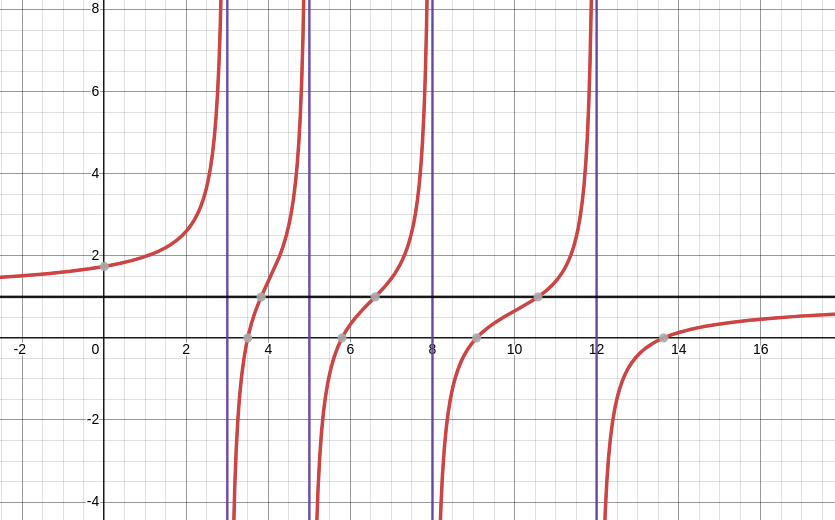
\includegraphics[scale=0.3]{img/f_lambda.png}

    \columnbreak

    Funkcja ta jest przedziałami rosnąca,\\
    $\qquad\lim_{\lambda \to d_i^+} f(\lambda) = -\infty$,\\
    $\qquad\lim_{\lambda \to d_i^-} f(\lambda) = +\infty$,\\
    $\qquad\lim_{\lambda \to -\infty} f(\lambda) = 1 = \lim_{\lambda \to \infty} f(\lambda)$\\

    Wynika z tego, że $f$ ma dokładnie jedno zero w $(d_i, d_{i+1})$
    dla $i=1...N-1$ oraz jedno miejsce zerowe na prawo od $d_N$.
\end{multicols}

Wiemy, że $B$ ma uporządkowane, różne wartości własne, więc kolejne miejsca zerowa $f$
odpowiadają właśnie im. Szukanie miejsc zerowych możemy wykonać z "dowolną" dokładnością
za pomocą metody Newtona, bisekcji lub dowolnej innej metody.

Wyznaczywszy wartość własną $B$, $\lambda_i$, odpowiadający jej wektor własny jest
równy $v_i = (D - \lambda_i I)^{-1}\cdot z$. Faktycznie
\begin{align*}
    (D + zz^T)\underbrace{(D - \lambda_i I)^{-1}z}_{v_i}                  & = \lambda_i \underbrace{(D - \lambda_i I)^{-1} z}_{v_i}                                                    \\
    Dv_i + zz^Tv_i                                                        & = \lambda_i v_i                                                                                            \\
    v_i = \left[\frac{z_j}{d_j - \lambda_i}\right]_{j=1..N}
    \qquad                                                                & \qquad
    Dv_i = \left[\frac{d_j z_j}{d_j - \lambda_i}\right]_{j=1..N}                                                                                                                       \\
    1+z^Tv_i = f(\lambda_i) = 0 \qquad                                    & \to \qquad z^Tv_i = -1                                                                                     \\
    \text{Dla ustalonego $j$ }\qquad\frac{d_j z_j}{d_j - \lambda_i} - z_j & = z_j \left(\frac{d_j - (d_j - \lambda_i)}{d_j - \lambda_i}\right) = \frac{z_j\lambda_i}{d_j - \lambda_i},
\end{align*}
więc $v_i$ jest odpowiadającym wektorem własnym. Otrzymane wektory układamy
w macierz i stosujemy wszystkie odpowiednie opisane powyżej przejścia.

\subsubsection*{Dowód Lematu (*)}
Lemat: $\det(I + yz^T) = 1 + y^T z$ przy założeniu, że $y, z \neq 0$
\\
Dowód: Znajdźmy wartości własne $I + yz^T$.
\begin{align*}
    (I + yz^T)x & = \lambda x \\
    Ix + yz^Tx  & = \lambda x \\
\end{align*}
Rozpatrzmy $x := y$. Wówczas $y + yz^Ty = \lambda y$, więc $y(1 + z^Ty - \lambda) = 0$, a skoro $y \neq 0$,
to $\lambda = 1 + z^Ty$, zatem $(y, 1 + z^Ty)$ jest parą własną.
\\
Rozpatrzmy $x \in (\text{span}\{z\})^{\perp}$. Wówczas $z^Tx = 0$, więc $x + yz^Tx = x = 1 x$, więc pozostałe wartości własne to 1.

\newpage
\section*{Zagadnienie 3}
Porównanie metod: standardowej metody Monte Carlo i quasi-Monte Carlo.

\subsection*{Rozumowanie}

Poniżej porównamy metody Monte Cargo i quasi-Monte Carlo. Obie te metody
służą do numerycznego obliczania całek. Całka, którą chcemy policzyć
ma postać
$$
    I_d(f) := \int_{D} f(x) dx, \qquad D = [0, 1]^d.
$$
i zakładamy, że $f : D \to \R$ jest całkowalna z kwadratem, t.j.
$
    \int_{D} |f(x)|^2 dx < \infty.
$

\subsubsection*{Klasyczna metoda Monte Carlo}
Klasyczna metoda Monte Carlo opisana jest wzorem
$$
    MC_{d, N}(f) = \frac{1}{N} \sum_{i=1}^{N} f(t_i) = MC_{d, N}(d, t_1, \dots, t_N),
$$
gdzie $t_1, \dots, t_N$ to niezależne zmienne losowe o rozkładzie jednostajnym na $D$.

W ramach wykładu wykazaliśmy, że metoda ma kilka problemów. Przede wszystkim
jej błąd jest rzędu $\mathcal{O}(N^{-\frac{1}{2}})$, co oznacza, że aby uzyskać
dokładność $\varepsilon$, musimy wykonać $\mathcal{O}(\varepsilon^{-2})$ iteracji.

Jako, że wartość oczekiwana $f$ jest równa $I_d(f)$, to polegamy na prawdopodobieństwie
i generatorach liczb losowych. Niestety generatory liczb losowych w komputerach
są tak naprawdę generatorami pseudolosowych, a zatem nie są w stanie wygenerować
liczb o rozkładzie jednostajnym.
W związku z tym wynik otrzymany za pomocą tej metody jest bardzo niepewny.

\subsubsection*{Metoda quasi-Monte Carlo}

Metoda quasi-Monte Carlo opisana jest wzorem
$$
    QMC_{d, N}(f) = \frac{1}{N} \sum_{i=1}^{N} f(t_i) = QMC_{d, N}(d, t_1, \dots, t_N),
$$
gdzie $t_1, \dots, t_N$ to pewne szczególne punkty w $D$.

Chcemy, aby te szczególne punkty były jak najbardziej równomiernie rozłożone,
więc zdefiniujemy pojęcie \textit{dyskrepancji}.

Dyskrepancją danego zbioru $N$ punktów $t_i \in D$ nazywamy
$$
    \text{DISC}_{d}(t_1, \dots, t_N) = \Pi_{k=1}^{d} x_k - \frac{\#\{ i : t_i \in [0, x) \} }{N}, \qquad
    x = (x_1, \dots, x_d) \in D.
$$
Z kolei dyskrepancją z gwiazdką nazywamy
$$
    \text{DISC}^*_{D}(t_1, \dots, t_N) = \sup_{x \in D} \; \text{DISC}_{d}(x, t_1, \dots, t_N).
$$

Wprowadzimy kilka pomocniczych oznaczeń:
\begin{enumerate}
    \item podzbiory indeksów $U$: $\emptyset \neq U \subseteq \{1, \dots, d\}$,
    \item $D_U = [0, 1]^{|U|}$,
    \item $x = [x_1, \dots, x_d]^T \in D$,
    \item $x_U \in D_U$ - wektor składający się z tych współrzędnych $x$, które odpowiadają indeksom z $U$,
    \item $(x_U; 1) \in D$ - wektor dla którego zachodzi $(x_U; 1)_j = x_j$ dla $j \in U$ oraz $(x_U; 1)_j = 1$ dla $j \notin U$.
    \item $f'_U = \frac{\partial^{|U|f}}{\Pi_{j\in U} \partial u_j}$ - pochodna cząstkowa funkcji $f$ po zmiennych o współrzędnych z $U$.
\end{enumerate}

Formuła Zaremby opisuje błąd metody quasi-Monte Carlo. Mianowicie $I_d(f) - QMC_{d, N}(f)$ wynosi
$$
    \sum_{U}(-1)^{|U|} \int_{D_U} \text{DISC}_d((z_U; 1), t_1, \dots, t_N) f'_N(z_U; 1)dz_U.
$$

Niech $\mathcal{V}_d(V)$ będzie klasą funkcji $f : D \to \R$, których pochodne cząstkowe
mieszane $f'_D$ istnieją i są ciągłe dla wszystkich $U$. Wówczas
wachaniem $f$ w sensie Hardy'ego-Krausego nazywamy
$$
    V_d(f) := \sum_{U} \int_{D_U} |f'(z_U;1)|dz_U.
$$

Co więcej, nierówność Koksmy-Hlawki mówi, że jeśli $f \in \mathcal{V}_d(V)$, to
błąd metody quasi-Monte Carlo szacuje się przez
$$
    |I_d(f) - QMC_{d, N}(f)| \leq V_d(f) \cdot \text{DISC}^*_{D}(t_1, \dots, t_N).
$$

Z tego właśnie powodu opłacalną strategią jest dobieranie ciągów punktów $t_1, \dots, t_N$
tak, aby były one o niskiej dyskrepancji z gwiazdką. Konkretnie ciągiem o niskiej
dyskrepancji nazwiemy nieskończony ciąg $t_1, t_2, \dots$, taki że istnieje
stała $D_d > 0$, że dla każdego $N$ zachodzi
$$
    \text{DISC}^*_{D}(t_1, \dots, t_N) \leq C_D \frac{\ln^{d}N}{N}.
$$

Rozważymy teraz kilka ciągów o niskiej dyskrepancji.

\subsubsection*{Ciąg van der Corputa}

Niech $b \in \N$ będzie ustaloną, większym od 1, liczbą naturalną.
Ciąg van der Corputa o podstawie $b$ to ciąg $t_1, t_2, \dots$ zdefiniowany
rekurencyjnie następująco:
$$
    t_n = \sum_{k=0}^{d} \frac{a_k}{b^{k+1}}, \qquad n = \sum_{k=0}^{d} a_k b^k, \qquad a_k \in \{0, \dots, b-1\}.
$$

\begin{multicols*}{2}
    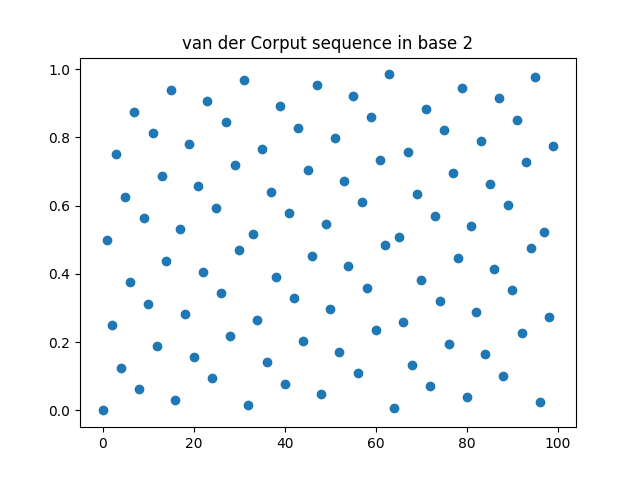
\includegraphics[scale=0.5]{img/corput.png}

    \columnbreak

    Algorytm wyznaczania $n$-tego wyrazu ciągu van der Corputa o podstawie $b$.
    \begin{lstlisting}
    def corput(n: int, b: int) -> float:
        n_inv = 0.
        b_inv = 1. / b
        while n > 0:
            n_inv += (n % b) * b_inv
            n //= b
            b_inv /= b
        return n_inv
    \end{lstlisting}
\end{multicols*}

\subsubsection*{Ciąg Haltona}

Ciąg Haltona to ciąg $t_1, t_2, \dots$ zdefiniowany następująco.
Niech $b$ będzie bazą. Rozważmy bazę $b = 2$. Dzielimy odcinek $[0, 1]$ na dwie,
cztery, osiem, szesnaście, itd. części. To da nam następujące ciągi
\begin{align*}
    1/2  & \quad                                                                            \\
    1/4  & \quad 3/4                                                                        \\
    1/8  & \quad 3/8 \quad 5/8 \quad 7/8                                                    \\
    1/16 & \quad 3/16 \quad 5/16 \quad 7/16 \quad 9/16 \quad 11/16 \quad 13/16 \quad 15/16.
\end{align*}

Ostatecznie $n$-ta liczba ciągu będzie liczbą $n$ w zapisie dwójkowym,
odwrócona i zapisana w postaci dziesiętnej. Analogicznie dla innych baz. Dzielimy
odcinek $[0, 1]$ na $b$ części, potem na $b^2$ części, itd.

\begin{multicols}{2}
    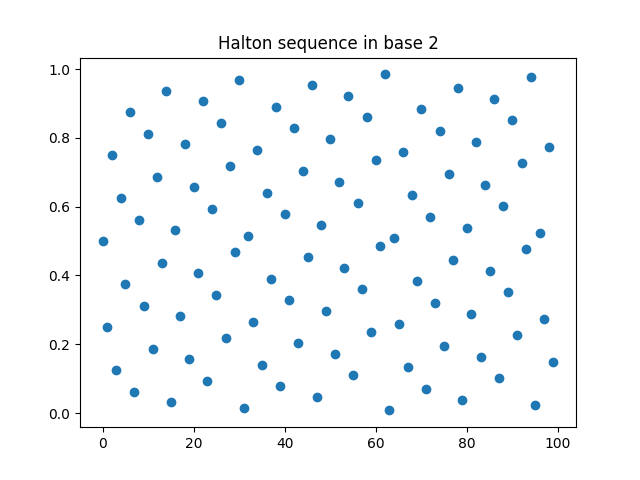
\includegraphics[scale=0.5]{img/halton.png}

    \columnbreak

    Algorytm wyznaczania ciągu Haltona za pomocą
    generatora w Pythonie:
    \begin{lstlisting}
    def halton_sequence(b: int) -> float:
        n, d = 0, 1
        while True:
            x = d - n
            if x == 1:
                n = 1
                d *= b
            else:
                y = d // b
                while x <= y:
                    y //= b
                n = (b + 1) * y - x
            yield n / d
    \end{lstlisting}
\end{multicols}

\subsubsection*{Eksperyment numeryczny -- błędy metody Monte Carlo i quasi-Monte Carlo}

Dla zadanej funkcji $f(x) = \sin(\pi x / 2) \cos(\pi x / 2) e^{-\sin^2(\pi x / 2)}$
na przedziale $D = [0, 1]$
oraz $N = 1000$ porównamy błędy metody Monte Carlo i quasi-Monte Carlo dla
ciągów van der Corputa i Haltona.
Na osi $x$ znajduje się numer iteracji (oraz liczba punktów), a na osi $y$
wartość bezwzględna błędu ze skalą logarytmiczną.
Dla zadanego $N$ ciągi van der Corputa i Haltona są deterministyczne,
ale metoda Monte Carlo jest losowa, więc rysowana jest dwa razy.
Raz dla pojedynczego losowania dla zadanego $x$, a raz dla średniej z 10 losowań.

\begin{multicols}{2}
    \begin{Figure}
        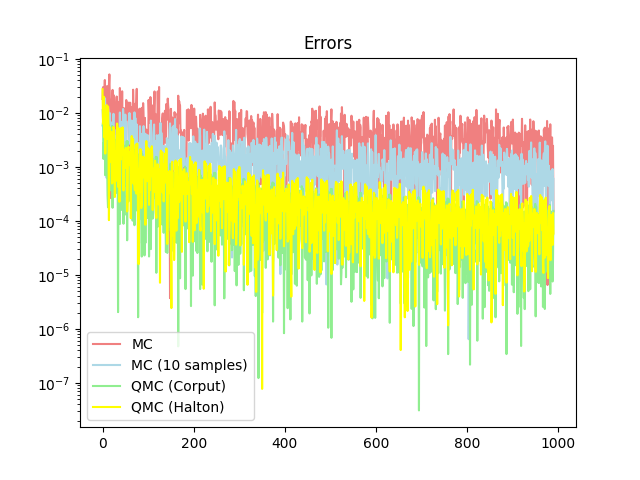
\includegraphics[scale=0.6]{img/errors.png}
        \centering
    \end{Figure}

    \columnbreak

    \begin{Figure}
        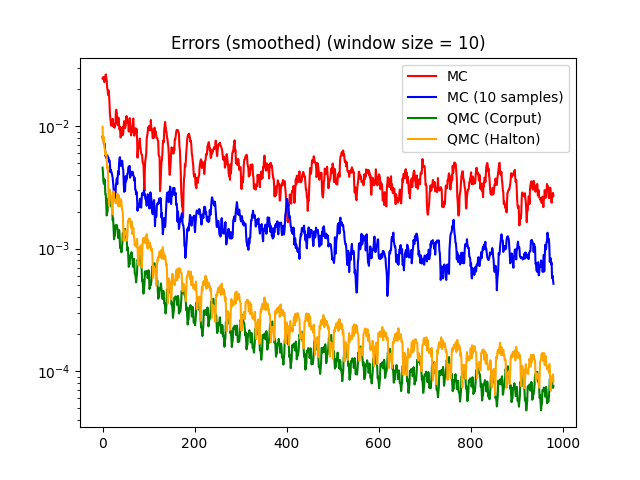
\includegraphics[scale=0.6]{img/errors_smoothed.png}
        \centering
    \end{Figure}
\end{multicols}

\end{document}

